% intro
Pixel-based reconstruction is an intuitive method to construct a volume from oriented ultrasound scans. In abstract sense, the scans are simply "inserted" into the volume. However, for a computer to this, a series of algorithmic steps needs to be devised. To obtain high performance, we can parallelize this algorithm and optimize the implementation. This section explains how pixel-based reconstruction is done in this thesis, including how this is parallelized and optimized for the GPU.

% description of the steps
\subsection{Method}

% (Fill compressed mask from mask)
% Fill pixel_ill from b-scans and mask
% Fill pixel_pos from mask
% Transform pixel_pos by pos_matrices
% Convert pixel_pos to volume indices
% Fill volume from pixel_pos and pixel_ill
% Fill holes of volume

	The method is based on pixel-nearest-neighbor (PNN) \cite{mccann1988}. The input is a set of $n$ b-scans images, a mask defining a region of interest (ROI) and $n$ tracking matrices. The b-scans are $w \times h$ arrays of grey-scale intensities, with 1 byte per pixel ($2^8=256$ possible values). The mask is the same format, where black is outside the ROI and white is inside, but there is only 1 mask for all $n$ b-scans. The tracking matrices are interpolated and calibrated using the $4 \times 3$ floating point transformation matrices as described in the previous section. The bottom row in the matrices will always be $(0,0,0,1)$, and is omitted.
	
	\begin{figure}[h]
	\centering
	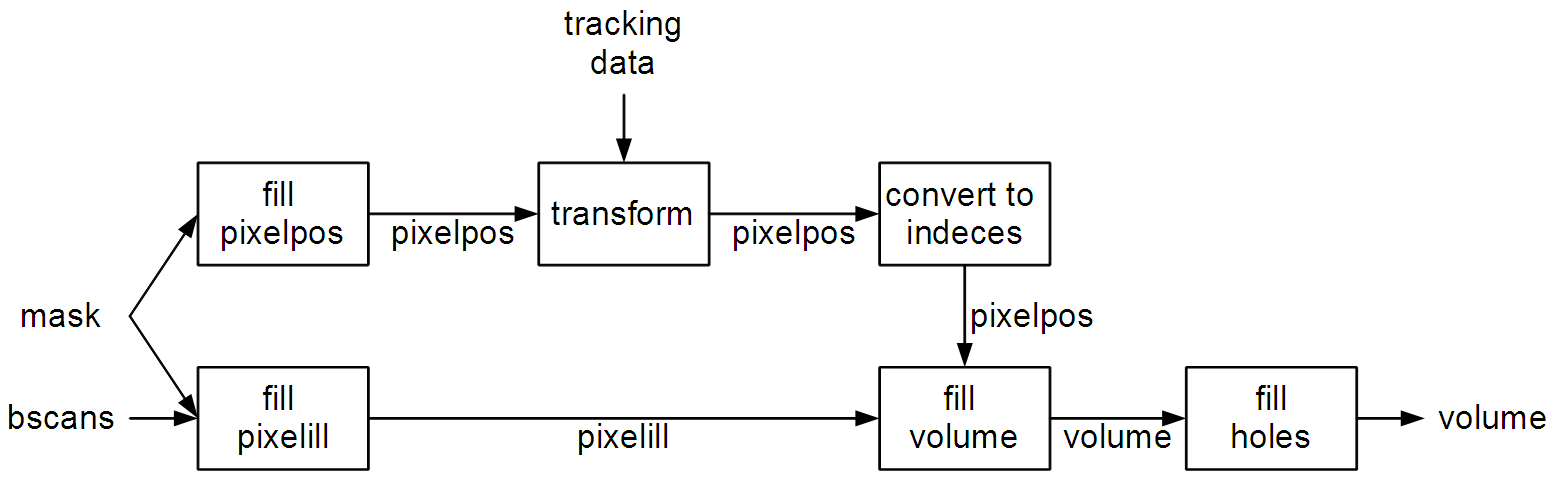
\includegraphics[width=\textwidth]{graphics/non-inc_pnn.png}
	\caption{Steps performed in pixel-based reconstruction}
	\label{fig:non-inc_pnn}
	\end{figure}
	
	There are 6 steps to be performed, resulting in the reconstructed volume. These steps are illustrated in Figure \ref{fig:non-inc_pnn} and given in the list below:
	
	\begin{enumerate}
		\item Fill $pixelpos$ from mask
		\item Fill $pixelill$ from b-scans and mask
		\item Transform $pixelpos$ by tracking matrices
		\item Convert coordinates to volume indices
		\item Fill volume from $pixelill$ and $pixelpos$
		\item Fill volume holes
	\end{enumerate}
	
	In the first step, we construct an array of three-dimensional coordinates, $pixelpos$, with one position for each pixel that is in the ROI in the mask. The coordinates are in world space, and are such that all the b-scans lie flat on the YZ-plane. This is given by Equation \ref{eq:pixelpos} where $i$ is the b-scan index (disregarded), $x$ and $y$ are the pixel indices, and $\Delta x$ and $\Delta y$ are the spacings between pixels in x- and y-direction (given as part of input). These coordinates are to be rotated by the tracking matrices to be positioned in the volume.
	
	\begin{equation}
	\label{eq:pixelpos}
		pixelpos(i,x,y) = (0, x\Delta x, y\Delta y)
	\end{equation}
	
	In the second step, the grey-scale intensities of the pixels in the ROI are saved as an array of bytes. The reason for doing this apparently redundant work is that the ROI can be much smaller than the entire b-scan. Typically, the scans are captured by a frame-grabber card connected to the ultrasound machine, and these images include metadata and empty space around the actual ultrasound data. The ROI is then just a fraction of the entire image. As an example, in the test data used in this thesis the ROI is 28 \% of the full scan. By extracting these into a separate array, we save memory, and there is a practical one-to-one mapping between pixel coordinates and pixel intensities.
	
	With this data ready, the transformation can begin in step three. For each b-scan, the corresponding tracking matrix is multiplied with the pixel coordinates to yield the coordinates in the volume. The operation is shown in Equation \ref{eq:transform_pixel_pos}. These coordinates are in world space, and in step four these are converted to volume indices by Equation \ref{eq:round_off} where $\Delta v$ is a given spacing between neighbor voxels. With the transformed coordinates converted to volume indices, the volume can be populated in step five. For each of the processed pixel coordinates, their corresponding pixel intensity is inserted into the volume using one of the possible compounding methods given in Table \ref{table:compounding_methods}. The effect of each specific method is given as an expression of the $old$ value present in the voxel and the $new$ value to be inserted.
	
	\begin{equation}
	\label{eq:transform_pixel_pos}
		pixelpos(i,x,y) := \bb{T}_i \cdot pixelpos(i,x,y)
	\end{equation}
	
	\begin{equation}
	\label{eq:round_off}
		pixelpos(i,x,y) := \Delta v \cdot pixelpos(i,x,y)
	\end{equation}
	
	\begin{table}[h]
	\centering
	\begin{tabular}{| l l l |}
		\hline
		\multicolumn{1}{|c}{\textbf{Method}} & \multicolumn{1}{c}{\textbf{Effect}} & \multicolumn{1}{c|}{\textbf{Condition}} \\
		\hline
		\hline
		average 			& $voxel \leftarrow \frac{old+new}{2}$ 	& old is not empty \\
		average 			& $voxel \leftarrow new$ 				& old is empty \\
		max 				& $voxel \leftarrow max(old, new)$ 		& \\
		ifempty 			& $voxel \leftarrow new$ 				& old is empty \\
		ifempty 			& $voxel \leftarrow old$ 				& old is not empty \\
		overwrite 			& $voxel \leftarrow new$ 				& \\
		\hline
	\end{tabular}
	\caption{Compounding methods}
	\label{table:compounding_methods}
	\end{table}
	
	The sixth and final step is to fill the volume holes. For each empty voxel, a $k \times k \times k$ kernel around it is averaged to give the voxel a value. In this kernel, only the non-empty voxels are considered for calculating the average, otherwise the filled holes would be darker than the surroundings. To save memory, hole filling is done in place, and thus there is a need for differentiating between actual holes and the empty voxel values before the first and after the last b-scan, in addition to those outside the region-of-interest. If every empty voxel would simply be filled, then non-empty voxels at the edges would be smudged out in the empty regions. This is resolved by counting the number of empty voxels in the kernel, and then only using the average to fill the hole if this number is above a cutoff value. An example cutoff value is $(k^3/2)-k$, which is slightly lower than half the number of voxels in the kernel. If the holes are not filled in place, e.g.\ by using a separate copy of the volume that has its holes filled, this cutoff is not necessary.

% description of how data/work is split up for parallelization,
% and also what parts are done on the CPU and GPU
\subsection{Parallelization}

%	Best practices guide p 31: multidimensional aspect of grid does not play a role in performance
%	Process input done on CPU because negligible
%	transfer b-scans and mask
%	?Generating pixel_pos and pixel_ill on GPU instead of transfer
%	NDRanges:
		%fill_pixel_ill_pos 	b-scan_n
		%transform 				b-scan_n x mask_size
		%round_off_translate	b-scan_n x mask_size
		%fill_volume			b-scan_n x mask_size
		%fill_holes				volume_w x volume_h x volume_n
%	Split b-scans and pixel_pos to overcome memory limits
%	transfer volume to CPU after processing

Code listings of the implemented OpenCL kernels can be found in Appendix \ref{section:pnn_kernel}. To parallelize the pixel-based reconstruction on the GPU, we need to divide the work into parts that can be performed simultaneously by many threads. To fully utilize the GPU, the number of work-items should in the order of hundreds of thousands or even millions \cite{bestpractices}. An elegant split of the work-domain will also ease the design of the kernels. OpenCL supports an \textit{NDRange} of up to three dimensions, but this multidimensional aspect does not play a role in overall performance \cite{bestpractices}, so this is not a consideration here.

Another task when parallelizing is to decide what parts to run on the highly parallel GPU and what parts to run on the relatively sequential CPU. There are additional overheads associated with doing work on the GPU, such as transferring data to and from the device memory and launching the kernel. The task of processing the input by calibration and interpolation is too small to be worth parallelizing for the GPU. However, each step in the reconstruction is parallelized.

After the input b-scans and tracking data has been transferred to the GPU memory, $pixelpos$ and $pixelill$ are generated and stored on the device. These arrays are only needed intermittently during reconstruction and thus never need to be transferred to or from the GPU. There are $n \times w \times h$ pixels that need to be processed into $n \times m$ coordinates in $pixelpos$, and intensities in $pixelill$, where $m$ is the number of pixels in the ROI. Dividing this into $n \times w \times h$ work-items is problematic because each work-item does not know where in the $pixelpos$ and $pixelill$ buffers to write when they find a ROI pixel. The solution is to evaluate $m$ on the CPU (negligible computation time), and give this as parameter to $n$ work-items that process a b-scan each. Each thread should generate $m$ elements, so a private counter is sufficient to manage where to write in memory.

The next three steps will process the $n \times m$ elements of $pixelpos$ and $pixelill$. The transformation task is divided into $n \times m$ work-items that each perform one matrix multiplication. The task of converting the coordinates to voxel indices and using them to fill the volume has the same number of work-items. For clarity however, these steps are not merged into one kernel. Filling the volume holes, on the other hand, is independent of the size of the input. The massive parallelism of the GPU allows for creating one work-item per voxel, totaling possibly millions, and where each work-item averages the neighbors if the voxel is empty. After this step, the volume is transferred back from the device if so desired. If the volume is visualized while on the GPU, this step might be skipped to save the transfer time.

%While commodity computers typically have 2 or more gigabytes of memory, GPUs found in current computers\footnote{Apple Mac Pro (2010)} can have only 512 megabytes. Some of this memory must be used by other applications, and the maximum

% description of various tricks and optimizations done
\subsection{Optimization techniques}

%	Good work group sizes with padding (big and multiple of 32)
%	Reduce variables to lower register usage
%	Compressed mask in constant memory
%	Transformation matrix in constant memory
%	Using constant memory for non-pointer arguments

In addition to increased performance from processing elements in parallel, there are further optimizations that can be performed. Actually, a naive porting of sequential code to the GPU does not necessarily utilize the device's capabilities, and might even result in a \emph{slowdown}. To make sure that each processing element in the device is occupied with work, we need to devise suitable work group sizes. As each work group is processed on one compute unit, we also need to ensure that its resources (such as shared memory) are not exhausted. On the CUDA architecture, groups (\emph{warps} in CUDA terminology) of 32 work elements are processed at the same time, so work group size should\footnote{In fact, if not multiple of 32, they will be padded to be so by CUDA.} be a multiple of 32. In order to hide memory latency, the total number of work groups should also be such that each compute unit have multiple groups to manage. On the Nvidia Tesla C2050 GPU, there are 16 compute units.

For the task of filling $pixelpos$ and $pixelill$, the \textit{NDRange} is only $n$ work-items, which is typically 200-500. To ensure enough work groups, we use a work group size of 32 and pad the \textit{NDRange} to a multiple of this work size. Such padding is generally done by Equation \ref{eq:padding}, where $p$ is the value of what $n$ should be a multiple of. The next steps have a substantially higher \textit{NDRange}, and we use work groups of 512 work-items which is the maximum possible size.

\begin{equation}
	\label{eq:padding}
	n_{padded} = (\lfloor \frac{n}{p} \rfloor + 1) \cdot p
\end{equation}

For further optimizations, the number of variables in the code is manually reduced to lower register usage and small data buffers are put in fast constant memory. The transformation matrices are small enough to fit without modifications, and by compressing the mask it too can fit. As mentioned, the mask uses the same format as the b-scans, with one byte per pixel. As the ROI is a boolean value (either in or out), eight pixels can be encoded into one byte using bitwise operations. This compression is performed on the CPU and also makes the mask faster to transfer to the device's memory.